\documentclass[main.tex]{subfiles}

\begin{document}

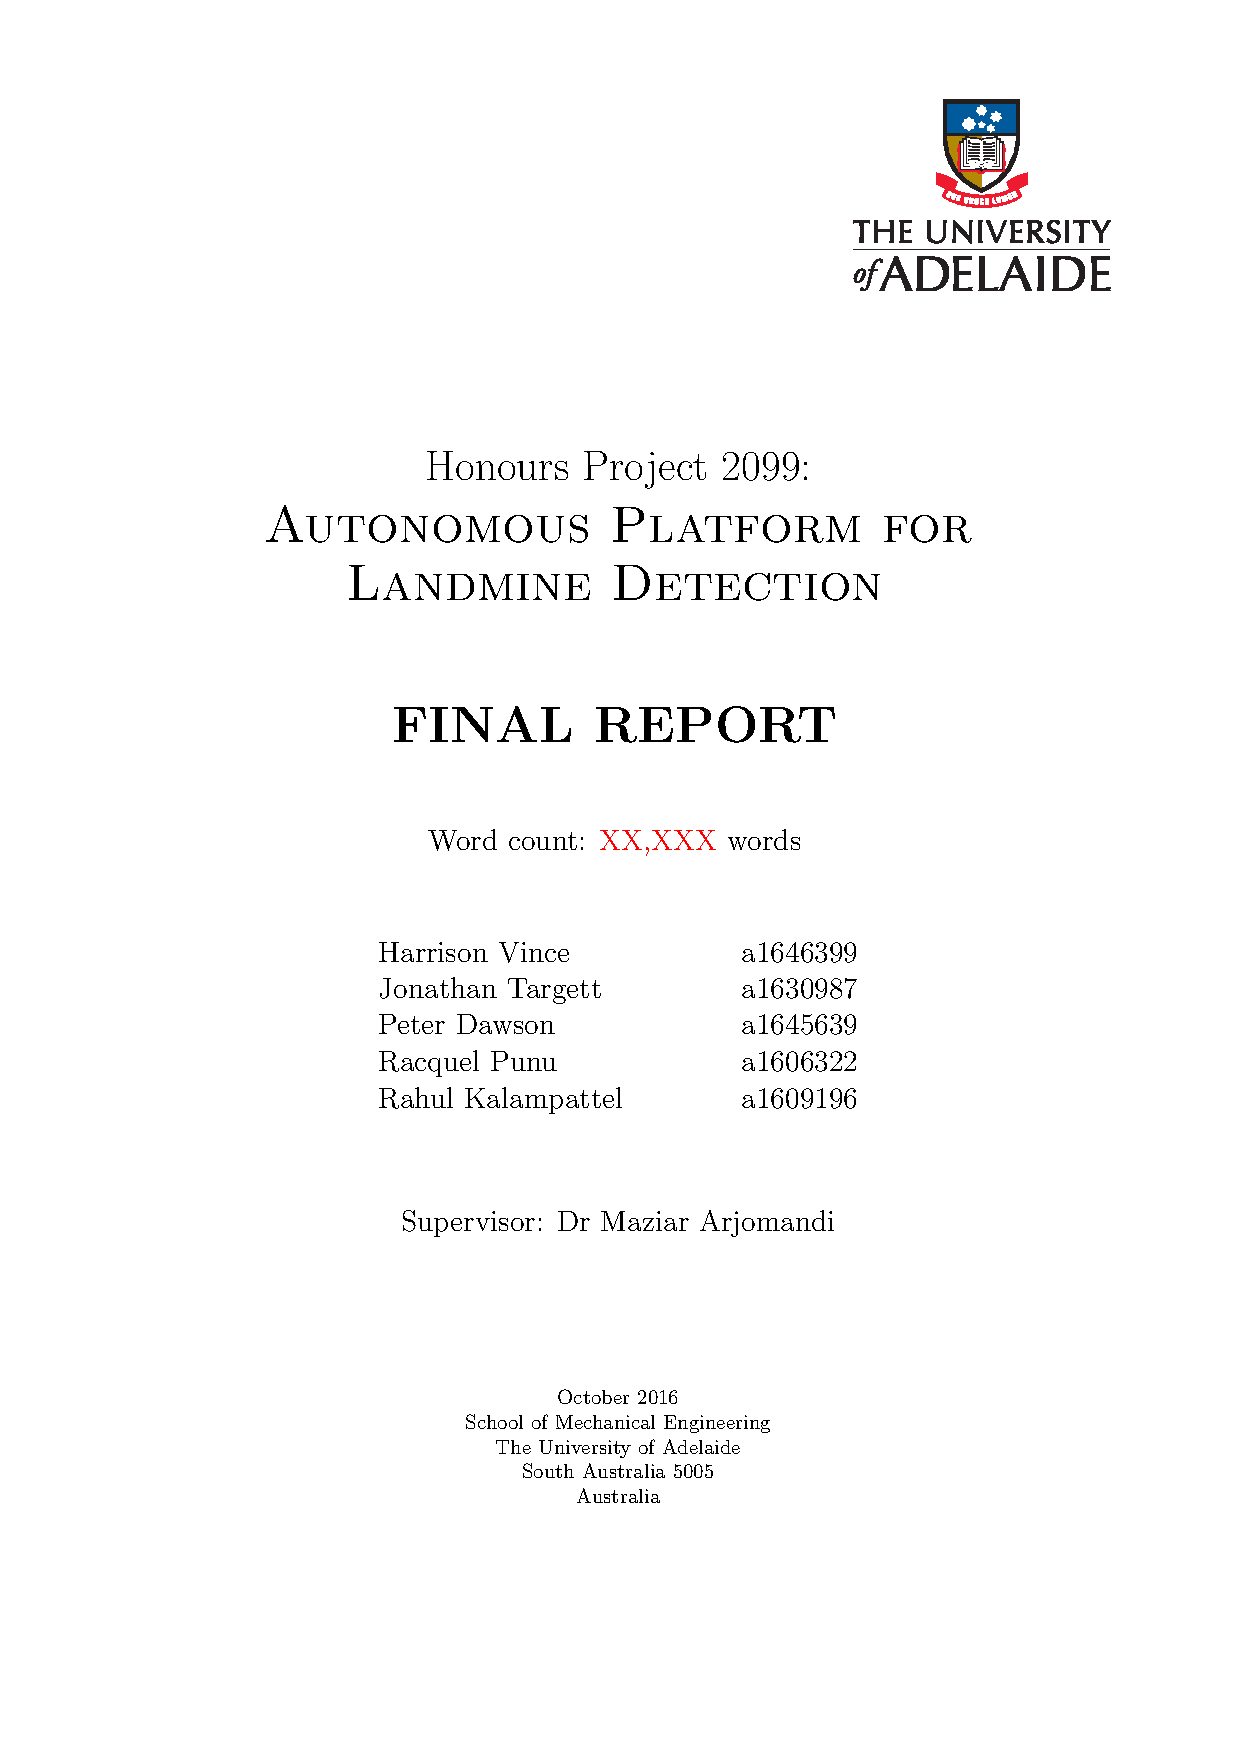
\includepdf{0-Preamble/coverpage.pdf}	% Get cover page (output from separate project)

\pagenumbering{roman}	% Numbering style for preamble
\phantomsection
\addcontentsline{toc}{chapter}{Executive Summary}	% Manually add ES to ToC
\chapter*{Executive Summary}
  
%This report gives an overview of the work completed for Honours Project 2099: Autonomous Platform for Landmine Detection. 

Landmines are indiscriminate weapons responsible for injuring thousands of civilians and military personnel every year. Current demining methods employed by groups such as the Australian Defence Force are inefficient and place operators at great risk. The major motivation for this project was to reduce this risk, and also to increase the speed of demining operations by reducing false positive detections. In collaboration with the Defence Science and Technology Group (DSTG), an autonomous and unmanned platform with a multisensor system for landmine detection was proposed as a solution. 

The primary objectives of the project were to modify a platform for automation, develop software for automation and basic navigation, develop software for navigating user defined paths, mount sensors on the platform and to develop software for landmine detection and classification. The extended objectives were to develop an accompanying tablet application, to provide a live video feed to the operator, and to physically mark the location of landmines. A scenario of operation was developed, outlining the operating environment and basic performance specifications for the platform and sensors. The scope of the project was limited to a proof of concept design.

Benchmarking was initially conducted to explore currently available platform and sensor options, and to better understand what the major challenges associated with the project would be. As part of the literature review, the development of techniques for signal processing, sensor fusion, automation and navigation were explored.        

A conceptual design process was undertaken to select subsystems and commence designs based on the requirements from the scenario of operation. A metal detector and ground penetrating radar (GPR) were chosen to be form the sensor suite, and a quad bike supplied by the DSTG was selected as the platform, since it already had the framework for automation implemented. Based on the chosen platform and sensors, design requirements and concepts were formed for the sensor mount. The final design sensor mount was chosen to provide minimal interference to the sensors while maximising the signal to noise ratio obtained. Preliminary tests with the sensors were used to identify metrics that could characterise landmines. The pure pursuit method was chosen for path tracking as it was most appropriate for the conditions expected to be encountered by the platform. For the electronics systems, an Arduino microcontroller was chosen to handle low level automation functions, while a desktop computer was selected as a central unit handling all communications and signal processing. 
%Development of software architecture for project. 

As part of the detailed design process, the ideas developed in the conceptual design were further refined. Algorithms for signal processing of sensor data were developed, as well as for sensor fusion, allowing for a confidence interval to be returned to an operator about the likelihood of a detected object being a landmine. Modifications were to made to key platform subsystems, namely the steering, brakes and gear subsystems. An Extended  Kalman Filter was used to fuse data from several positional sources, providing a positioning system with the necessary accuracy. Software for navigation and automation were developed, and preliminary testing was carried out in a virtual environment. A tablet application was also developed, allowing an operator to control the platform remotely and view the sensor data in real time. A structural and vibrational analysis of the sensor mount was performed, after which the mount was manufactured. The mount was made out of structural pine, with two steel supports to add extra stiffness. Due to the requirement to use non-metallic materials near the metal detector, nylon rods and perspex sheets were used to hold the metal detector in place.    

Testing was carried out to ensure that all subsystems were functioning as intended. Sensors tests were performed in two soil types with dummy landmines and clutter objects, and the data collected was used to build a database of metrics for automatic target identification. Tests of the positioning and other quad bike systems were also carried out, resulting in the fine tuning of electrical control subsystems. Communication difficulties resulted in unpredictable behaviour from the Arduino, which led to safety concerns. As a result, integrated systems testing is yet to be conducted. 

\textcolor{red}{The project management chapter gives an overview of the various management aspects of the project}, including the work breakdown structure and Gantt chart, risk management and the budget. 
All of the primary objectives, namely platform automation,  software for basic and user defined navigation, software for the sensor systems, and the design of the sensor mount have been completed. Of the extended objectives, a tablet application has been developed, however the provision of a live video feed and physical marking of landmine locations have not been implemented, presenting the opportunity for future work. 

\newpage
\phantomsection
\addcontentsline{toc}{chapter}{Disclaimer}	% Manually add ES to ToC
\chapter*{Disclaimer}
As the authors of this report, we declare that the material contained within is entirely our own work, unless otherwise specified. All work from other sources has been referenced accordingly. 
\vspace{0.4in}

% Update with correct images for signatures when ready, change dates as well

\noindent\begin{tabular}{ll}
\raisebox{-0.4in}[0pt][0pt]{
\includegraphics[height=0.7in]{0-Preamble/Harry.png}}&\raisebox{-0.0in}{24/10/2016}\\
\makebox[2.5in]{\hrulefill} & \makebox[1.4in]{\hrulefill}\\
Harrison Vince & Date\\[0.4in]% adds space between the two sets of signatures
\raisebox{-0.3in}[0pt][0pt]{
\includegraphics[height=0.5in]{0-Preamble/Jono.png}}&\raisebox{-0.0in}{24/10/2016}\\
\makebox[2.5in]{\hrulefill} & \makebox[1.4in]{\hrulefill}\\
Jonathan Targett & Date\\[0.4in]% adds space between the two sets of signatures
\raisebox{-0.4in}[0pt][0pt]{
\includegraphics[height=0.7in]{0-Preamble/Peter.PNG}}&\raisebox{-0.0in}{24/10/2016}\\
\makebox[2.5in]{\hrulefill} & \makebox[1.4in]{\hrulefill}\\
Peter Dawson & Date\\[0.4in]% adds space between the two sets of signatures
\raisebox{-0.4in}[0pt][0pt]{
\includegraphics[height=0.7in]{0-Preamble/Racquel.png}}&\raisebox{-0.0in}{24/10/2016}\\
\makebox[2.5in]{\hrulefill} & \makebox[1.4in]{\hrulefill}\\
Racquel Punu & Date\\[0.4in]% adds space between the two sets of signatures
\raisebox{-0.4in}[0pt][0pt]{
\includegraphics[height=0.7in]{0-Preamble/Rahul.jpg}}&\raisebox{-0.0in}{24/10/2016}\\
\makebox[2.5in]{\hrulefill} & \makebox[1.4in]{\hrulefill}\\
Rahul Kalampattel & Date
\end{tabular}
\newpage

\phantomsection
\addcontentsline{toc}{chapter}{Acknowledgements}	% Manually add ToC to ToC
\chapter*{Acknowledgements} 
The authors of this report acknowledge the contribution of several parties, without whom this project would not have been possible.

Firstly, the authors would like to thank the project sponsor, the Defence Science and Technology Group. As well as providing funding and equipment, the technical insights shared by Dr Canicious Abeynayake and his colleagues of the Weapons Effects \& Protection group are greatly appreciated. 

The authors also acknowledge the help of Kyle Blay from CSIRO and Greg Harmer from Minelab, both of whom provided invaluable assistance in understanding the sensor systems.

At the University of Adelaide, Rob Dempster, Phil Schmidt and several other members of both the Mechanical Engineering and Electronics and Instrumentation Workshops were responsible for helping out on numerous occasions. The authors also thank Marc Simpson at Thebarton Labs for allowing the use of lab facilities. 

Finally, the authors would like to thank Dr Maziar Arjomandi, the project supervisor, for his support, guidance and feedback throughout the year. 
\newpage

\phantomsection
\addcontentsline{toc}{chapter}{Contents}	% Manually add ToC to ToC
\renewcommand{\baselinestretch}{1.2}\normalsize 	% 1.2 line spacing
\tableofcontents
\renewcommand{\baselinestretch}{1.3}\normalsize 	% 1.3 line spacing
\newpage

\phantomsection
\addcontentsline{toc}{chapter}{List of Figures}	% Manually add LoF to ToC 
\listoffigures
\newpage

\phantomsection
\addcontentsline{toc}{chapter}{List of Tables}	% Manually add LoT to ToC
\listoftables
\newpage

% Uncomment the three lines below to split nomenclature into two columns
% \renewcommand*{\nompreamble}{\begin{multicols}{2}}
% \renewcommand*{\nompostamble}{\end{multicols}}
% \setlength{\columnsep}{3em}

\renewcommand{\nomname}{List of Acronyms}
\printnomenclature
\newpage

\end{document}